\documentclass[10pt,a4paper]{article}
\usepackage[utf8]{inputenc}
\usepackage{amsmath}
\usepackage{amsfonts}
\usepackage{amssymb}
\usepackage[left=2cm,right=2cm,top=2cm,bottom=2cm]{geometry}
\setlength{\oddsidemargin}{0.25 in}
\setlength{\evensidemargin}{-0.25 in}
\setlength{\topmargin}{-0.6 in}
\setlength{\textwidth}{6.5 in}
\setlength{\textheight}{8.5 in}
\setlength{\headsep}{0.75 in}
\setlength{\parindent}{0 in}
\setlength{\parskip}{0.1 in}

\usepackage{graphicx}
\usepackage{url}
\usepackage{multicol}
\usepackage{listings}
\usepackage[utf8]{inputenc}
\usepackage{amsmath}
\usepackage{amsfonts}
\usepackage{amssymb}
%\usepackage{graphicx}
\usepackage[left=2cm,right=2cm,top=2cm,bottom=2cm]{geometry}


\title{TyPy: A Python Bytecode Interpreter for the Browser}
\author{Puja Mishra, Kate Silverstein}
\date{27 October 2014}

\begin{document}
\maketitle
\section{Understanding the Requirements}

The goal of this project is to implement a Python bytecode interpreter which is engine dependent and also can be hosted on a variety of browsers. So the high level picture of how we have implemented is shown below in Figure 1.

\begin{figure}[ht!]
\caption{System Overview}
\centering
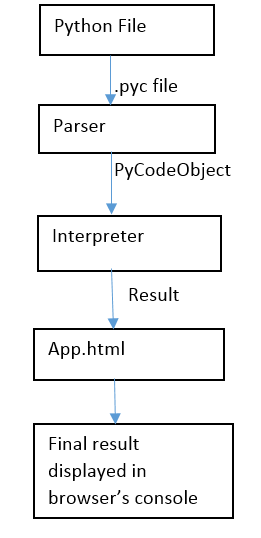
\includegraphics[scale=0.8]{../Report/UnderstandingTheReq.png} 
\end{figure}

\section{Design Approach}

The input to the system is the python program written by the user and compiled using "compileall" module. This *.pyc file is uploaded when the user opens application, this file is passed to the parser where parser parses the bytecodes and generates a PyCodeObject to the the interpreter (which here is a stack based interpreter) , which interprets it and gives the result on the browser's console.



\subsection{Parser}
% general structure of parser taken from UnPyc

\subsubsection{Structure of a Python Bytecode File}
The bytecode is an attribute of the code object and is found in cocode attribute of the code object and contains instructions for the interpreter. Bytecode is nothing but a series of bytes.The interpreter will loop through each byte, look up what it should do for each one, and then do that thing. Using the dis module we can disassemble the bytecode.


% \subsection{Character Encoding Considerations} (if there's time?)

\subsection{Interpreter Design}
The "standard" Python interpreter -- i.e. the one that ships with most distributions of Python -- is CPython, a "stack-based interpreter" written in C. There don't seem to be many alternatives to CPython: according to the CPython website, the main two are \emph{PyPy}, a Python implementation using a just-in-time compiler; and \emph{Stackless Python}, which is apparently not a stack-based implementation (however, the \emph{Stackless} website doesn't provide much detail other than that it "supports microthreads"). In addition, CPython has been re-implemented to run on both .NET and the JVM. 

The abundance of resources available for CPython ended up being the primary driver behind our decision to essentially port the relevant parts of CPython into Typescript. In the end, we borrowed the general structure of our interpreter from \emph{byterun} \cite{byterun}, a Python bytecode interpreter written in pure Python (which is, in turn, loosely based on \emph{CPython}, but much easier to read). Many aspects of \emph{byterun} translated into Typescript easily, while others did not (e.g. we had to completely re-implement anything that used a Python function from Python's built-in function library).

It is worth noting here that we could have instead chosen from several alternative approaches: a \emph{PyPy}-style JIT compiler, a "register-based" interpreter, or we could have made up something completely new. Since neither of the authors had written an interpreter before, however, we decided to go for "tried-and-true"; in the future, it may be worthwhile to explore alternative approaches.

\subsection{Other Design Considerations}
\subsubsection{Client-Side Javascript and Typescript} 

The requirement that our interpreter run entirely client-side required some thought. First, the basic challenge of loading a Python bytecode file into the browser's local storage system posed some difficulty. Second, we had to design our program to work with client-side Javascript's asynchronous nature. Third, we had to figure out how to allow "importing" code asynchronously in order to keep our code modular and apply good software engineering design practices.

% have to store files in browser local storage
% have to use BrowserFS instead Node.js
% have compile using AMD module instead of commonjs module (why did this matter? what are differences?)
% have to use RequireJS to import

%\subsection{Test Suite}
% CORS request to test server (Express)

\section{Implementation Results}
\subsection{Supported Functionality}
The interpreter we have implemented can interpret simple "if" statements, for and while loops, basic list creation and indexing, basic dictionary creation and queries, basic math operations.
% sample output from browser console

% \subsection{Runtime and Efficiency} %(if there's time)
% how long does it take to run e.g. sorting a list for a huge list?

\section{Future Work}
As an extension of the project we can add more functionality which can help to interpret complex functions written in python.

\section{Conclusion}
Working on this project has been a very good and learning  experience. The system implemented by us is a simple interpreter which can interpret basic functionality written in python.

\begin{thebibliography}{9}

\bibitem{byterun}
  Ned Batchelder,
  \emph{byterun }.
  https://github.com/nedbat/byterun

\bibitem{unpyc}
Dmitri Kornev
\emph{UnPyc}.
Dmitri Kornev

\bibitem{brocious}
Cody Brocious
"Python Marshal Format." \emph{I, Hacker}. 20 February 2010.

\end{thebibliography}




\end{document}


